\section{Modul Bebas}\label{sec:free-modules}
Tetap tetapkan gelanggang $R$. Berikutnya kita meninjau konstruksi ``bebas'' dalam kategori modul $R\dcate{Mod}$. Misalkan $X$ suatu himpunan (kecil). Untuk setiap $x \in X$, definisikan modul siklik $Rx$ sebagai berikut: unsur-unsurnya adalah simbol berbentuk $rx$, dengan $r \in R$; penjumlahan dan perkalian skalarnya masing-masing didefinisikan oleh $rx + r'x = (r+r')x$, $r(r'x) = (rr')x$. Dengan kata lain, sebagai modul kiri atas $R$, $Rx$ sebenarnya hanyalah $R$, tetapi secara formal ditambahi simbol $x$ di sebelah kanan.
\begin{definition}\label{def:free-module}\index{modul!bebas (free module)}
	\emph{Modul bebas} dengan basis $X$ didefinisikan sebagai $R^{\oplus X} = \bigoplus_{x \in X} Rx$. Sebagai himpunan, terdapat peta inklusi alami
	\begin{align*}
		X & \longrightarrow R^{\oplus X} \\
		x & \longmapsto 1 \cdot x.
	\end{align*}
	Unsur-unsurnya dapat ditulis sebagai jumlah berhingga $m = \sum_{x \in X} a_x x$ atau larik $(a_x)_{x \in X}$, dengan $a_x \in R$ ditentukan secara tunggal dan paling banyak berhingga banyak di antaranya tak nol; notasi ini konsisten dengan notasi yang diperkenalkan dalam pembuktian Teorema \ref{prop:module-cat-completeness}.
\end{definition}
Ini adalah definisi ekstrinsik modul bebas dan basisnya; versi intrinsiknya akan diberikan segera. Mudah dilihat bahwa $X \mapsto R^{\oplus X}$ mendefinisikan fungtor $\cate{Set} \to R\dcate{Mod}$ yang dicirikan oleh sifat universal berikut.

\begin{proposition}\label{prop:free-module-property}
	Untuk setiap $R$-modul $M$ dan peta himpunan $\phi: X \to M$, terdapat tepat satu homomorfisme modul $\varphi: R^{\oplus X} \to M$ yang membuat diagram berikut komutatif.
	\[ \begin{tikzcd}
		X \arrow[rd, "\phi"'] \arrow[r] & R^{\oplus X} \arrow[d, "{\exists! \, \varphi}"] \\
		& M
	\end{tikzcd} \]
\end{proposition}
\begin{proof}
	Jelas bahwa untuk setiap $x \in X$ harus berlaku $\varphi(rx) = r\varphi(x) = r\phi(x) \in M$; hal ini menentukan $\varphi$ sepenuhnya.
\end{proof}
Jadi, fungtor $X \mapsto R^{\oplus X}$ adalah fungtor adjoin kiri bagi fungtor pelupa; dengan kata lain, terdapat isomorfisme natural
\[ \Hom_R(R^{\oplus X}, M) \rightiso \Hom_\cate{Set}(X, M), \]
dengan peubah $X$ merentang semua himpunan dan $M$ merentang semua $R$-modul. Dari sudut pandang lain, memberikan homomorfisme yang berawal dari $R^{\oplus X}$ ekuivalen dengan menentukan bayangan setiap unsur basis $X$ tanpa syarat apa pun; karena itulah konstruksi ini ``bebas''.

Pada kesempatan ini, kita memperumum beberapa konsep yang lazim dalam aljabar linear ke modul.
\begin{definition}
	Misalkan $X$ suatu subhimpunan dari $R$-modul $M$. Menurut Proposisi \ref{prop:free-module-property}, peta inklusi $X \hookrightarrow M$ menginduksi homomorfisme $\sigma: R^{\oplus X} \to M$. Kita katakan bahwa
	\begin{itemize}
		\item $X$ \emph{bebas linear} atau \emph{bebas} jika $\sigma$ injektif; jika tidak, $X$ disebut \emph{bergantung linear};
		\item $X$ membangkitkan atau merentang $M$ jika $\sigma$ surjektif; dalam hal ini $X$ disebut \emph{himpunan pembangkit} bagi $M$. Modul yang mempunyai himpunan pembangkit berhingga disebut \emph{modul yang dibangkitkan secara berhingga}.\index{dibangkitkan secara berhingga}
	\end{itemize}
	Himpunan pembangkit yang bebas linear disebut \emph{basis}; modul yang memiliki basis juga disebut \emph{modul bebas}. Ini adalah versi intrinsik Definisi \ref{def:free-module}.
\end{definition}
Perhatikan bahwa $\sigma$ injektif ekuivalen dengan $\Ker(\sigma)=\{0\}$, yang sama artinya dengan
\[ \underbracket{\sum_{x \in X} r_x x}_{M\text{ dalam jumlah berhingga}} = 0 \iff \forall x \in X, \; r_x = 0. \]
Sementara itu, $\sigma$ surjektif ekuivalen dengan setiap unsur dapat ditulis sebagai kombinasi linear atas $R$, $\sum_{x \in X} r_x x$. Ini semua adalah definisi yang dikenal dari aljabar linear. Jelas bahwa $X$ adalah basis dari $R^{\oplus X}$; jadi definisi intrinsik dan ekstrinsik modul bebas selaras.

Sebagai contoh, misalkan $\Delta$ suatu monoid. Pembaca dapat memeriksa bahwa gelanggang monoid $R[\Delta]$ yang dibangun dalam Definisi \ref{def:monoidal-ring}, dengan aksi perkalian kiri oleh $R$ yang diberikan oleh $r\cdot(\sum_{\delta \in \Delta} r_\delta \delta) = \sum_{\delta \in \Delta} rr_\delta \delta$ (dengan $r \in R$), merupakan modul kiri atas $R$, dan bahwa $\Delta \subset R[\Delta]$ adalah basis. Kasus perkalian kanan serupa. Sebagai kasus khusus, gelanggang polinomial $R[X] = \bigoplus_{n \geq 0 }RX^n$ adalah modul kiri bebas atas $R$ dengan basis $\Delta := \{ X^n: n \geq 0 \}$.

\begin{corollary}
	Hingga isomorfisme, setiap modul $M$ dapat dinyatakan sebagai hasil bagi suatu modul bebas.
\end{corollary}
\begin{proof}
	Ambil suatu subhimpunan $X$ dari $M$ dan homomorfisme terkait $\sigma: R^{\oplus X} \to M$. Maka $\Image(\sigma) \simeq R^{\oplus X}/\Ker(\sigma)$. Jika $X$ dipilih sebagai himpunan pembangkit bagi $M$ (misalnya $X=M$), maka $\Image(\sigma)=M$.
\end{proof}

Jika basis $X$ berhingga, gelanggang endomorfisme $R^{\oplus X}$ dapat dinyatakan sebagai gelanggang matriks yang dikenal dari Contoh \ref{eg:matrix-ring}. Tanpa mengurangi keumuman, anggap $X = \{1, \ldots, n\}$. Kita mulai dengan produk berhingga umum dalam $\cated{Mod}R$; kuncinya adalah menerapkan Korolari \ref{prop:Mod-cat-additive}. Sesungguhnya, argumen berikut berlaku dalam sebarang kategori aditif (Definisi \ref{def:additive-cat}). Pilih
\begin{compactitem}
	\item bilangan bulat positif $n, m$;
	\item objek $M_1, \ldots, M_n$ dan $M'_1, \ldots, M'_m$.
\end{compactitem}
Di sini $\bigoplus_{i=1}^n M_i$ sekaligus berperan sebagai produk langsung dan jumlah langsung, yang masing-masing diberikan oleh dua keluarga morfisme $\bigoplus_{i=1}^n M_i \xrightarrow{p_j} M_j$ dan $M_j \xrightarrow{\iota_j} \bigoplus_{i=1}^n M_i$. Demikian pula terdapat morfisme $p'_j, \iota'_j$, dan seterusnya. Maka, dari sifat universal produk dan koproduk,
\begin{align*}
	\Hom \left( \bigoplus_{j=1}^n M_j, \bigoplus_{i=1}^m M'_i \right) & \xrightarrow[\sim]{\phi \mapsto (p'_i \phi)_i } \prod_{i=1}^m \Hom\left(\bigoplus_{j=1}^n M_j , M'_i \right) \\
	& \xrightarrow[\sim]{(p'_i \phi)_i \mapsto (p'_i \phi \iota_j)_{i, j}} \prod_{j=1}^n \prod_{i=1}^m  \Hom(M_j, M'_i).
\end{align*}
Jadi, $\phi: \bigoplus_{j=1}^n M_j \to \bigoplus_{i=1}^m M'_i$ sepenuhnya ditentukan oleh keluarga homomorfisme
\[ \phi_{ij} := p'_i \phi \iota_j: M_j \to M'_i, \quad 1 \leq i \leq m, \; 1 \leq j \leq n \]
dan direpresentasikan oleh matriks
\[ \phi \longleftrightarrow \mathcal{M}(\phi) = (\phi_{ij})_{\substack{1 \leq i \leq m \\ 1 \leq j \leq n}} = \begin{pmatrix}
	\phi_{11} & \cdots & \phi_{1n} \\
	\vdots & \ddots & \vdots \\
	\phi_{m1} & \cdots & \phi_{mn} 
\end{pmatrix}. \]
Ingat bahwa perkalian matriks $C=AB$ ditentukan oleh $c_{ik} = \sum_j a_{ij} b_{jk}$. Untuk matriks $\mathcal{M}(\phi)$, meskipun unsur-unsurnya mengambil nilai dalam grup-grup aditif $\Hom$ yang mungkin berbeda, operasi yang digunakan berikut ini tetap terdefinisi dengan baik.

\begin{lemma}\label{prop:Hom-matrix}
	Untuk $\phi: \bigoplus_{i=1}^n M_i \to \bigoplus_{i=1}^{n'} M'_i$ dan $\psi: \bigoplus_{i=1}^{n'} M'_i \to \bigoplus_{i=1}^{n''} M''_i$, matriks-matriks terkait memenuhi
	\[ \mathcal{M}(\psi\phi) = \mathcal{M}(\psi) \mathcal{M}(\phi) \]
	dengan perkalian unsur matriks diberikan oleh komposisi $\Hom(M'_j, M''_i) \times \Hom(M_k, M'_j) \to \Hom(M_k, M''_i)$.
\end{lemma}
\begin{proof}
	Gunakan persamaan $\sum_{j=1}^{n'} \iota'_j p'_j = 1$, $p'_i \iota'_i = \identity_{M'_i}$, dan $i \neq j \implies p'_i \iota'_j = 0$ dalam gelanggang $\End_R(\bigoplus_i M'_i)$ (versi banyak peubah dari Definisi \ref{def:biproduct}) untuk menghitung koefisien matriks ke-$(i, k)$, $\mathcal{M}(\psi\phi)_{ik}$, dari $\psi\phi$. Berdasarkan asosiativitas dan bilinearitas komposisi homomorfisme, diperoleh
	\begin{align*}
		\mathcal{M}(\psi\phi)_{ik} = p''_i \psi\phi \iota_k & = \sum_{j=1}^{n'} p''_i \psi (\iota'_j p'_j) \phi \iota_k \\
		& = \sum_{j=1}^{n'} (p''_i \psi \iota'_j) (p'_j \phi \iota_k) = \sum_{j=1}^{n'} \mathcal{M}(\psi)_{ij} \mathcal{M}(\phi)_{jk}.
	\end{align*}
	Ini tepat merupakan perkalian matriks, sehingga pernyataan terbukti.
\end{proof}

Argumen di atas persis sejajar dengan cara merepresentasikan transformasi linear oleh matriks dalam aljabar linear.
\begin{proposition}\label{prop:End-matrix}
	Gelanggang endomorfisme modul $R^{\oplus n}$ secara alami isomorfik dengan gelanggang matriks $n \times n$, $M_n(R^\text{op})$; isomorfisme ini diinduksi oleh $\phi \mapsto \mathcal{M}(\phi)$. Lebih lanjut, grup aditif $\Hom_R(R^{\oplus n}, R^{\oplus m})$ secara alami isomorfik dengan grup aditif semua matriks $m \times n$, $M_{m \times n}(R^\text{op})$; komposisi homomorfisme bersesuaian dengan perkalian matriks.
	
	Jika kita memakai modul kanan atas $R$, maka secara bersesuaian diperoleh $\Hom_R(R^{\oplus n}, R^{\oplus m}) \simeq M_{m \times n}(R)$.
\end{proposition}
\begin{proof}
	Pandang $R$ sebagai modul kiri atas $R$, dan tulis ${}_R R$. Setiap $\phi \in \End({}_R R)$ memenuhi $\phi(r) = r\phi(1)$; dari sini dapat dibuktikan bahwa
	\begin{align*}
		\End({}_R R) & \longrightarrow R^\text{op} \\
		\phi & \longmapsto \phi(1)
	\end{align*}
	merupakan isomorfisme gelanggang. Inversnya memetakan $r \in R$ ke endomorfisme perkalian kanan $x \mapsto xr$ (perhatikan bahwa urutan perkalian berbalik). Substitusikan $M_i = M'_j = {}_R R$ dalam pembahasan sebelumnya dan Lemma \ref{prop:Hom-matrix} untuk memperoleh pernyataan. Untuk modul kanan, berlaku $\End(R_R) \simeq R$, dan sisanya sama.
\end{proof}

``Lemma pembangkit'' berikut melibatkan kardinal tak hingga yang diperkenalkan secara singkat dalam \S\ref{sec:cardinal-number}.
\begin{lemma}\label{prop:generator-cardinal}
	Misalkan $I$ suatu himpunan tak hingga dan $(M_i)_{i \in I}$ suatu keluarga modul tak nol. Setiap himpunan pembangkit $S$ dari $\bigoplus_{i \in I} M_i$ memenuhi $|S| \geq |I|$.
\end{lemma}
\begin{proof}
	Setiap $s \in S$ dapat ditulis sebagai $(s_i)_{i \in I}$; tulis $E_s := \{i \in I: s_i \neq 0\}$. Menurut definisi jumlah langsung, $E_s$ berhingga, sedangkan fakta bahwa $S$ membangkitkan $\bigoplus_{i \in I} M_i$ menyiratkan $\bigcup_{s \in S} E_s = I$; karena itu $S$ tak hingga. Korolari \ref{prop:cardinal-max} lalu memberikan ketaksamaan kardinal
	\[ \max\{|S|, \aleph_0 \} = |S| \cdot \aleph_0 \geq \left| \bigcup_{s \in S} E_s \right| = |I|, \]
	dan ruas paling kiri tidak lain adalah $|S|$.
\end{proof}

Terakhir, kita membahas rank modul bebas. Dalam uraian berikut, anggap $R$ tak nol. Gagasan alaminya ialah mendefinisikan rank $M \simeq R^{\oplus X}$ sebagai $|X|$, tetapi harus ditunjukkan bahwa nilai ini tidak bergantung pada pilihan basis $X \subset M$. Bila $R$ suatu medan, teori ruang vektor menunjukkan bahwa rank memang terdefinisi dengan baik. Pembaca tentu telah mengenal kasus berdimensi hingga, sedangkan Definisi--Teorema \ref{def:dimension-vector-space} akan memberikan pembuktian umum dengan menggunakan Lemma \ref{prop:generator-cardinal}. Dari sini kita dapat menurunkan sifat serupa bagi modul bebas atas gelanggang komutatif.

\begin{proposition}
	Misalkan $R$ suatu gelanggang komutatif. Maka $R^{\oplus X} \simeq R^{\oplus Y}$ jika dan hanya jika $|X|=|Y|$.
\end{proposition}
\begin{proof}
	Jelas bahwa $|X|=|Y|$ menyiratkan $R^{\oplus X} \simeq R^{\oplus Y}$. Untuk membuktikan arah sebaliknya, terapkan Proposisi \ref{prop:existence-maximal-ideal} untuk memilih suatu ideal maksimal $\mathfrak{m}$ dari $R$. Bagi setiap $R$-modul $M$, definisikan $\mathfrak{m} M$ sebagai submodul yang dibangkitkan oleh semua unsur berbentuk $am$ ($m \in M$, $a \in \mathfrak{m}$). Maka $M/\mathfrak{m}M$ adalah modul atas $R/\mathfrak{m}$, yakni ruang vektor atas medan $R/\mathfrak{m}$. Bila $M = R^{\oplus X}$, mudah dilihat bahwa $\mathfrak{m}M = \mathfrak{m}^{\oplus X}$; dengan demikian terdapat isomorfisme ruang vektor
	\begin{align*}
		M/\mathfrak{m}M & \stackrel{\sim}{\longrightarrow} (R/\mathfrak{m})^{\oplus X} \\
		(a_x)_{x \in X} + \mathfrak{m}M & \longmapsto (a_x + \mathfrak{m})_{x \in X}.
	\end{align*}
	Jadi $|X| = \dim_{R/\mathfrak{m}} (M/\mathfrak{m}M)$, dan ruas kanan hanya bergantung pada struktur $R$-modul dari $M$, bukan pada pilihan basis.
\end{proof}

\begin{definition}[Rank modul bebas]\label{def:rank-module}\index[sym1]{rank@$\rank_R(E)$}\index{rank@rank (rank)}
	Misalkan $E$ suatu modul bebas atas gelanggang komutatif tak nol $R$. \emph{Rank}-nya didefinisikan sebagai $\rank_R(E) := |X|$ jika $E \simeq R^{\oplus X}$. Menurut proposisi sebelumnya, ini terdefinisi dengan baik.
\end{definition}

\begin{remark}\label{rem:IBN}
	Untuk gelanggang umum $R$, jika $I$ suatu himpunan tak hingga dan $R^{\oplus I} \simeq R^{\oplus J}$, maka Lemma \ref{prop:generator-cardinal} menyiratkan $|J| \geq |I|$; oleh simetri, $|I|=|J|$. Jadi modul bebas atas gelanggang $R$ mempunyai rank yang terdefinisi dengan baik jika dan hanya jika
	\[ \forall n,m \in \Z_{\geq 0}, \; R^{\oplus n} \simeq R^{\oplus m} \iff n=m. \]
	Ini disebut sifat \emph{bilangan basis invarian} kiri (disingkat IBN dalam bahasa Inggris); untuk modul kanan, disebut sifat bilangan basis invarian kanan. Gelanggang pembagian, gelanggang komutatif, dan gelanggang berhingga semuanya mempunyai sifat bilangan basis invarian. Untuk pembahasan lebih lanjut, lihat \cite[\S 1]{Lam99}.
\end{remark}

\section{Ruang Vektor}\label{sec:vector-space}
Pembaca semestinya telah mengenal teori ruang vektor. Dari sudut pandang aljabar, ruang vektor pada dasarnya adalah struktur yang dilengkapi penjumlahan dan perkalian skalar; skalar biasanya berasal dari medan bilangan real $\R$ atau medan bilangan kompleks $\CC$. Namun, sifat-sifat aljabarnya sebenarnya dapat dikembangkan atas sebarang medan. Kita bahkan dapat meninggalkan komutativitas perkalian dan meninjau ruang vektor atas gelanggang pembagian. Perumuman ini alami dan mudah, serta diperlukan dalam kajian teori gelanggang.

\begin{definition}\index{ruang vektor@ruang vektor (vector space)}
	Misalkan $D$ suatu gelanggang pembagian. Modul kanan atas $D$ disebut \emph{ruang vektor} atas $D$. Submodul dan modul hasil baginya masing-masing juga disebut subruang dan ruang hasil bagi.
\end{definition}
Pilihan modul kiri atau kanan dalam definisi pada dasarnya tidak penting; bila $D$ suatu medan, sisi tindakan bahkan tidak perlu disebutkan. Kita memilih perkalian kanan demi kemudahan notasi: jika $\varphi: V \to V'$ suatu morfisme ruang vektor atas $D$ (yakni morfisme modul kanan atas $D$), sifat morfisme terhadap perkalian skalar dapat ditulis menyerupai hukum asosiatif:
\[ \varphi (vd) = (\varphi v)d, \quad v \in V, \; d \in D. \]

Selanjutnya tetapkan gelanggang pembagian $D$. Konsep subruang, basis, dimensi, dan sebagainya dapat diperumum ke ruang vektor atas $D$ tanpa kesulitan.

\begin{definition-theorem}\index{basis@basis (basis)}
	Misalkan $V$ suatu ruang vektor atas $D$ dan $X \subset V$. Sifat-sifat berikut ekuivalen:
	\begin{enumerate}[(i)]
		\item $X$ adalah subhimpunan bebas linear maksimal dari $V$;
		\item peta inklusi $X \hookrightarrow V$ menginduksi isomorfisme $D^{\oplus X} \rightiso V$;
		\item $X$ adalah himpunan pembangkit minimal dari $V$;
		\item setiap unsur $V$ dapat ditulis sebagai jumlah berhingga berbentuk $\sum_{x \in X} x d_x$, dengan $(d_x)_{x \in X}$ tunggal.
	\end{enumerate}
	Himpunan $X$ yang memenuhi salah satu sifat di atas disebut \emph{basis} dari $V$.
\end{definition-theorem}
\begin{proof}
	(i) $\implies$ (ii): Diberikan $v \in V$, maksimalitas $X$ menyiratkan bahwa $X \sqcup \{v\}$ bergantung linear. Karena itu terdapat persamaan $\sum_{x \in X \sqcup \{v\}} x d_x = 0$ dengan tidak semua $d_x$ nol. Kebebasan linear $X$ menyiratkan $d_v \neq 0$, sehingga $v = -\sum_{x \in X} x d_x d_v^{-1}$ berada dalam bayangan $D^{\oplus X} \to V$. Karena $D^{\oplus X} \to V$ injektif, peta ini merupakan isomorfisme.

	(ii) $\implies$ (iii): Tanpa mengurangi keumuman, anggap $V = D^{\oplus X}$. Jelas bahwa $X$ membangkitkan $V$. Jika $X' \subset X \smallsetminus \{y\}$ (dengan $y \in X$), maka jelas $y$ tidak termasuk submodul $D^{\oplus X'}$ yang dibangkitkan oleh $X'$; jadi $X$ adalah himpunan pembangkit minimal.

	(iii) $\implies$ (iv): Karena $X$ membangkitkan $V$, setiap unsur dapat ditulis sebagai jumlah berhingga $\sum_{x \in X} x d_x$. Jika
	\[ \sum_{x \in X} x d_x = \sum_{x \in X} x d'_x, \quad \exists y \in X, \; d_y \neq d'_y, \]
	maka $y = -\sum_{x \neq y} x (d_x - d'_x)(d_y - d'_y)^{-1}$, sehingga $X \smallsetminus \{y\}$ juga membangkitkan $V$, suatu kontradiksi.

	(iv) $\implies$ (i): Subhimpunan $X$ jelas bebas linear. Setiap $v \in V$ dapat ditulis sebagai $\sum_{x \in X} x d_x$, yaitu $v - \sum_{x \in X} x d_x = 0$; oleh karena itu $X \sqcup \{v\}$ bergantung linear.
\end{proof}

\begin{proposition}\label{prop:existence-basis}
	Setiap subhimpunan bebas linear $X$ dari $V$ termuat dalam suatu basis $B$; khususnya, $V$ mempunyai basis.
\end{proposition}
\begin{proof}
	Tetapkan $X$ dan definisikan $\mathcal{E} := \{Y \subset V: \text{bebas linear}, \; Y \supset X  \}$, lalu berikan $\mathcal{E}$ urutan parsial $Y \leq Y' \iff Y \subset Y'$. Kita menerapkan Lemma Zorn (Teorema \ref{prop:Zorn}) untuk membuktikan bahwa poset $(\mathcal{E}, \leq)$ mempunyai unsur maksimal dan dengan demikian memperoleh basis yang dicari. Cukup dibuktikan bahwa setiap rantai $\mathcal{E}'$ dalam $(\mathcal{E}, \leq)$ mempunyai batas atas. Misalkan $Y \subset V$ adalah gabungan semua unsur $\mathcal{E}'$. Kita menyatakan bahwa $Y$ bebas linear: andaikan persamaan
	\[ \sum_{y \in Y} y d_y = 0 \quad \text{(jumlah berhingga)} \]
berlaku. Karena $\mathcal{E}'$ terurut total, dapat dipilih $Y_0 \in \mathcal{E}'$ yang cukup besar sehingga $y \notin Y_0 \implies d_y = 0$. Kebebasan linear $Y_0$ lalu memberikan $\forall y \in Y, \; d_y = 0$. Jadi $Y$ adalah batas atas yang dicari.
\end{proof}

\begin{lemma}[Sifat pertukaran Steinitz]\label{prop:exchange-vector-space}
	Misalkan $X$, $Y$ dua basis berhingga dari $V$ dan $y \in Y \smallsetminus X$. Maka terdapat $x \in X \smallsetminus Y$ sehingga $(Y \smallsetminus \{y\}) \cup \{x\}$ merupakan basis.
\end{lemma}
\begin{proof}
	Perhatikan bahwa ketakosongan $X$ menjamin ketakosongan $Y$. Setiap $x \in X$ mempunyai pengembangan tunggal sebagai kombinasi linear atas $D$ dari $Y$. Kita menyatakan bahwa $y$ harus muncul dalam pengembangan suatu $x$; jika tidak, $Y \smallsetminus \{y\}$ akan menjadi himpunan pembangkit bagi $V$, bertentangan dengan definisi basis. Pilih $x$ demikian dan definisikan $Z := (Y \smallsetminus \{y\}) \cup \{x\}$. Perhatikan bahwa
	\begin{inparaenum}[(a)]
		\item setiap unsur $Y$ dapat dikembangkan sebagai kombinasi linear dari $Z$; untuk kasus $y$, gunakan pengembangan $x$;
		\item $Z$ harus bebas linear: jika tidak, karena $Y \smallsetminus \{y\}$ bebas linear, $x$ dapat ditulis sebagai kombinasi linear dari $Y \smallsetminus \{y\}$. Bersama langkah sebelumnya, ini menyiratkan bahwa $y$ juga dapat ditulis sebagai kombinasi linear dari $Y \smallsetminus \{y\}$, suatu kontradiksi.
	\end{inparaenum}
	Jadi, setiap unsur $V$ dapat ditulis secara tunggal sebagai kombinasi linear dari $Z$. Terakhir, perhatikan bahwa $x \notin Y$: jika tidak, $y \notin X \implies y \neq x \implies Z = Y \smallsetminus \{y\}$, bertentangan dengan sifat basis sebagai subhimpunan bebas linear maksimal.
\end{proof}

Sifat pertukaran adalah kunci untuk membuktikan bahwa dimensi terdefinisi dengan baik. Karena argumen serupa muncul di banyak tempat dalam aljabar, kita sekaligus memperkenalkan perangkat kombinatorial berikut.
\begin{definition}[H.\ Whitney]\label{def:matroid}\index{matroid@matroid (matroid)}
	Misalkan $E$ suatu himpunan dan $\text{Bs}$ suatu keluarga subhimpunan berhingga dari $E$. Data $(E, \text{Bs})$ disebut \emph{matroid} jika syarat-syarat berikut dipenuhi:
	\begin{enumerate}[\bfseries {B}.1]
		\item Himpunan $\text{Bs}$ tidak kosong;
		\item jika $X, Y \in \text{Bs}$ dan $y \in Y \smallsetminus X$, maka terdapat $x \in X \smallsetminus Y$ sehingga $(Y \smallsetminus \{y\}) \cup \{x\}\; \in \text{Bs}$.
	\end{enumerate}
\end{definition}
Sebagai contoh, jika ruang vektor $V$ atas $D$ mempunyai suatu basis berhingga, Lemma \ref{prop:generator-cardinal} menyiratkan bahwa setiap basisnya berhingga. Dalam hal ini, dengan menerapkan Lemma \ref{prop:exchange-vector-space} serta mengambil $E := V$ dan $\text{Bs} := \{ V\;\text{ basis} \}$, kita memperoleh sebuah matroid. Definisi umum biasanya juga mensyaratkan $E$ berhingga, tetapi hal ini tidak penting di sini. Daya tarik matroid adalah adanya berbagai karakterisasi yang ekuivalen tetapi tampak sangat berbeda. Pembaca yang berminat dapat melihat monograf \cite{Oxl11}. 

\begin{proposition}\label{prop:matroid-rank}
	Misalkan $(E, \mathrm{Bs})$ suatu matroid. Setiap unsur $\mathrm{Bs}$ mempunyai kardinalitas yang sama; kardinalitas ini disebut rank matroid tersebut.
\end{proposition}
\begin{proof}
	Andaikan tidak demikian. Pilih $X, Y \in \text{Bs}$ dengan $|Y| > |X|$ dan $|Y \smallsetminus X|$ sekecil mungkin. Syarat pertama menjamin $Y \smallsetminus X \neq \emptyset$. Menurut sifat pertukaran (\textbf{B.2}), dapat dipilih $y \in Y \smallsetminus X$ dan $x \in X \smallsetminus Y$ sehingga $Y' := (Y \smallsetminus \{y\}) \cup \{x\}\; \in \text{Bs}$. Dari $|Y|=|Y'| > |X|$ dan $|Y' \smallsetminus X| < |Y \smallsetminus X|$ diperoleh kontradiksi.
\end{proof}

\begin{definition-theorem}[Keinvarian dimensi]\label{def:dimension-vector-space}\index[sym1]{dim@$\dim$}\index{ruang vektor!dimensi (dimension)}
	Misalkan $X, Y$ dua basis dari $V$. Maka $|X|=|Y|$. Dengan demikian, \emph{dimensi} $V$ dapat didefinisikan sebagai kardinalitas $|X|$ dan ditulis $\dim V$ atau $\dim_D V$, dengan $X$ sebarang basis dari $V$.
\end{definition-theorem}
\begin{proof}
	Seperti diamati sebelumnya, Lemma \ref{prop:generator-cardinal} menyiratkan bahwa semua basis $V$ berhingga atau semuanya tak hingga. Dalam kasus tak hingga, berlaku $|X| \leq |Y| \leq |X|$; Teorema \ref{prop:Schröder-Bernstein} segera memberikan $|X|=|Y|$.

	Jika semua basis $V$ berhingga, terapkan struktur matroid dan Proposisi \ref{prop:matroid-rank} untuk memperoleh $|X|=|Y|$.
\end{proof}
Dalam \S\ref{sec:free-modules}, hasil ini digunakan untuk membuktikan bahwa modul bebas atas gelanggang komutatif tak nol mempunyai rank yang terdefinisi dengan baik.
 
\section{Hasil Kali Tensor Modul}\label{sec:module-tensor-prod}
Hasil kali tensor adalah salah satu konstruksi yang paling sering digunakan dalam teori modul. Mari mulai dari kasus ruang vektor yang dikenal: misalkan $X, Y$ ruang vektor atas $\CC$, dan tinjau fungsi $B: X \times Y \to A$ dengan nilai dalam suatu ruang vektor $A$ atas $\CC$. Jika $B(x, \cdot)$ dan $B(\cdot, y)$ merupakan peta linear untuk semua $x,y$, maka $B$ disebut bentuk bilinear. Hasil kali tensor $X$ dan $Y$ tidak lain adalah ``bentuk bilinear universal'' $X \times Y \to X \dotimes{\CC} Y$. Lebih tepatnya, kita menuntut agar setiap bentuk bilinear $B: X \times Y \to A$ dapat difaktorkan sebagai
$\begin{tikzcd}[row sep=small, column sep=small]
	X \times Y \arrow[r] \arrow[rd, "B"'] & X \dotimes{\CC} Y \arrow[d, "\exists! \, f"] \\
	& A
\end{tikzcd}$
dengan $f$ peta linear yang ditentukan secara tunggal. Tanpa terlebih dahulu membahas konstruksinya, tulis bayangan $(x,y) \in X \times Y$ dalam $X \dotimes{\CC} Y$ sebagai $x \otimes y$. Bilinearitas menyiratkan
\begin{gather*}
	(x+x') \otimes y = x \otimes y + x' \otimes y, \quad x \otimes (y+y') = x \otimes y + x \otimes y', \\
	(tx) \otimes y = t(x \otimes y) = x \otimes (ty), \quad t \in \CC.
\end{gather*}
Secara wajar, ruang vektor $X \dotimes{\CC} Y$ harus direntang oleh semua $x \otimes y$, dan $X \dotimes{\CC} Y$ tidak memiliki kendala lain selain sifat-sifat di atas; jika tidak, ia tidak lagi ``universal''.

Untuk modul umum, rumusan masalahnya tidak berbeda, tetapi diperlukan serangkaian persiapan, dimulai dengan konsep bimodul.
\begin{definition}[Bimodul]\index{bimodul@bimodul (bimodule)}
	Misalkan $R, S$ gelanggang. Sebuah \emph{bimodul} $(R, S)$ adalah grup aditif $M$ yang sekaligus mempunyai struktur modul kiri atas $R$ dan modul kanan atas $S$, serta memenuhi
	\[ r(ms) = (rm)s, \quad m \in M, \; r \in R, \; s \in S. \]
\end{definition}
Ungkapan dalam persamaan ini dapat ditulis singkat sebagai $rms$. Ia dapat dipahami sebagai sejenis hukum asosiatif perkalian maupun sebagai kekomutatifan antara perkalian kiri oleh $R$ dan perkalian kanan oleh $S$. Bagi bimodul $(R, S)$, konsep homomorfisme, isomorfisme, modul hasil bagi, dan sebagainya didefinisikan dengan jelas; dengan demikian diperoleh kategori bimodul $(R, S)\dcate{Mod}$. Catatan \ref{rem:bimodule-as-module} akan menjelaskan cara mereduksi teori bimodul ke kasus satu sisi.

\begin{example}\label{eg:bimodule-Z}
	Terdapat isomorfisme kategori $R\dcate{Mod} \simeq (R, \Z)\dcate{Mod}$. Alasannya, setiap modul kiri $M$ atas $R$ mempunyai struktur perkalian kanan oleh $\Z$ yang tunggal, yaitu $ma := am$, dengan $m \in M$, $a \in \Z$, dan aksioma bimodul jelas dipenuhi. Demikian pula, $\cated{Mod}R \simeq (\Z, R)\dcate{Mod}$.
\end{example}

\begin{example}\label{eg:bimodule-comm}
	Jika $R$ komutatif, setiap modul kiri $M$ atas $R$ secara alami menjadi bimodul $(R, R)$: cukup definisikan $rmr' := rr' m$.
\end{example}

\begin{convention}\index[sym1]{R_M_S@${}_R M_S$}
	Selanjutnya kita akan sesekali memakai notasi ${}_R M$ (atau $M_S$, ${}_R M_S$) untuk menyatakan bahwa $M$ dilengkapi struktur modul kiri atas $R$ (atau modul kanan atas $S$, bimodul $(R, S)$).
\end{convention}

Bahasa bimodul memudahkan kajian hasil kali tensor. Hasil kali tensor dicirikan oleh sifat universal sebagai sejenis ``hasil kali seimbang'', yakni versi nonkomutatif bentuk bilinear. Kita mulai dengan hasil kali seimbang yang mengambil nilai dalam suatu grup abelian $A$; kasus ketika $A$ merupakan bimodul akan dibahas dalam Catatan \ref{rem:bimodule-balanced}.

\begin{definition}[Hasil kali seimbang: kasus satu sisi]\label{def:balanced-product}\index{hasil kali seimbang@hasil kali seimbang (balanced product)}
	Misalkan $R$ suatu gelanggang. Tinjau modul $M_R$, ${}_R N$, dan grup abelian $(A, +)$. Suatu peta
	\[ B: M \times N \to A \]
	disebut \emph{hasil kali seimbang} jika memenuhi syarat-syarat berikut:
	\begin{compactenum}[(i)]
		\item $B(x+x', y) = B(x, y) + B(x', y)$,
		\item $B(x, y+y') = B(x, y) + B(x, y')$,
		\item $B(xr, y) = B(x, ry)$,
	\end{compactenum}
	dengan $x, x' \in M$, $y, y' \in N$, dan $r \in R$ sebarang unsur. Himpunan semua hasil kali seimbang $B: M \times N \to A$ ditulis $\text{Bil}(M, N; A)$ dan membentuk grup abelian terhadap penjumlahan.
\end{definition}

Untuk $M$, $N$ yang diberikan, semua hasil kali seimbang yang berawal dari $M \times N$ membentuk kategori $\cate{Bil}(M, N; \ast)$. Morfisme dari objek $B$ ke $B'$ didefinisikan sebagai diagram komutatif berbentuk
\[ \begin{tikzcd}[row sep=tiny]
	{} & A \arrow[dd, "\text{homomorfisme grup}"] \\
	M \times N \arrow[ru, "B"] \arrow[rd, "B'"'] & \\
	& A'
\end{tikzcd} \]

Hasil kali tensor $M \times N \to M \dotimes{R} N$ yang akan segera didefinisikan tidak lain adalah objek awal dari $\cate{Bil}(M, N; \ast)$; lihat Definisi \ref{def:universal-objects}.

\begin{definition}\label{def:tensor-product}\index{hasil kali tensor@hasil kali tensor (tensor product)}\index[sym1]{1otimes}
	Hasil kali seimbang $M \times N \to M \dotimes{R} N$ yang memenuhi sifat universal berikut disebut \emph{hasil kali tensor} dari $M_R$ dan ${}_R N$: untuk setiap hasil kali seimbang $B: M \times N \to A$, terdapat tepat satu homomorfisme grup $M \dotimes{R} N \to A $ yang membuat diagram berikut komutatif:
	\[ \begin{tikzcd}[row sep=small]
		M \times N \arrow[rd, "B"'] \arrow[r] & M \dotimes{R} N \arrow[d, "\exists!"] \\
		& A
	\end{tikzcd} \]
\end{definition}
Karena $M \times N \to M \dotimes{R} N$ dicirikan oleh sifat universal, ia ditentukan secara tunggal hingga isomorfisme tunggal. Biasanya kita menghilangkan panah dan cukup menyebut $M \dotimes{R} N$ sebagai hasil kali tensor $M$ dan $N$; terkadang indeks $R$ pada $\otimes$ juga dihilangkan. Bayangan unsur $(x, y)$ dalam $M \dotimes{R} N$ ditulis $x \otimes y$. Perhatikan bahwa membahas struktur $M \dotimes{R} N$ semata tidak terlalu bermakna; ketika menyelidiki berbagai sifat fungtorial hasil kali tensor di bawah ini, peta $(x, y) \mapsto x \otimes y$ harus selalu ikut diperhitungkan.

\begin{lemma}
	Untuk setiap $M_R$, ${}_R N$, terdapat hasil kali tensor $M \times N \to M \dotimes{R} N$.
\end{lemma}
\begin{proof}
	Terinspirasi oleh pembahasan pada awal bagian ini, tinjau modul bebas $F$ atas $\Z$ pada himpunan $M \times N$. Unsur-unsur berbentuk
	\begin{gather*}
		(x + x', y) - (x, y) - (x', y) \\
		(x, y + y') - (x, y) - (x, y') \\
		(xr, y) - (x, ry)
	\end{gather*}
	membangkitkan suatu submodul $I$ atas $\Z$. Tulis $M \dotimes{R} N := F/I$, dan tulis bayangan $(x,y) \in M \times N$ dalam $F/I$ sebagai $x \otimes y$. Kita akan membuktikan bahwa peta $M \times N \to M \dotimes{R} N$ ini adalah yang dicari.

	Menurut definisi modul bebas, memberikan grup abelian $A$ dan peta $B: M \times N \to A$ ekuivalen dengan memberikan homomorfisme $\beta: F \to A$, dengan korespondensi yang ditentukan secara tunggal oleh
	\[ \beta(x,y) = B(x,y), \quad (x,y) \in M \times N \]
	Jadi, $B$ adalah hasil kali seimbang jika dan hanya jika $\beta$ nol pada $I$. Sebagai kasus khusus, $M \times N \to F/I$ juga merupakan hasil kali seimbang. Dalam keadaan ini, misalkan $\bar{\beta}: F/I \to A$ homomorfisme yang diinduksi oleh $\beta$. Korespondensi antara hasil kali seimbang $B: M \times N \to A$ dan homomorfisme $\bar{\beta}: M \dotimes{R} N \to A$ dicirikan oleh
	\[ \bar{\beta}(x \otimes y) = B(x,y) \]
	dan persamaan ini ekuivalen dengan kekomutatifan diagram dalam Definisi \ref{def:tensor-product}.
\end{proof}

\begin{lemma}\label{prop:functoriality-tensor}
	Hasil kali tensor $M \dotimes{R} N$ bersifat fungtorial dalam $M, N$: jika $\varphi: M \to M'$ dan $\psi: N \to N'$ adalah homomorfisme modul, maka terdapat tepat satu homomorfisme $\varphi \otimes \psi: M \dotimes{R} N \to M' \dotimes{R} N'$ yang membuat diagram berikut komutatif.
	\[ \begin{tikzcd}
		M \times N \arrow[r] \arrow[d, "{\varphi \times \psi}"'] & M \dotimes{R} N \arrow[d, "{\exists! \varphi \otimes \psi}"] \\
		M' \times N' \arrow[r] & M' \dotimes{R} N'
	\end{tikzcd} \]
\end{lemma}
\begin{proof}
	Peta komposit $M \times N \xrightarrow{\phi \times \psi} M' \times N' \to M' \dotimes{R} N'$ jelas juga merupakan hasil kali seimbang. Definisi \ref{def:tensor-product} kemudian memberikan tepat satu $\varphi \otimes \psi: M \dotimes{R} N \to M' \dotimes{R} N'$ yang membuat diagram di atas komutatif.
\end{proof}
Syarat dalam lemma di atas ekuivalen dengan
\[ (\varphi \otimes \psi) (x \otimes y) = \varphi(x) \otimes \psi(y). \]
Syarat ini menentukan homomorfisme $\varphi \otimes \psi$ secara tunggal. Dari karakterisasi ini, hasil kali tensor homomorfisme kompatibel dengan komposisi homomorfisme:
\[ (\varphi \otimes \psi) \circ (\varphi' \otimes \psi') = (\varphi \circ \varphi') \otimes (\psi \circ \psi'), \]
dengan syarat bahwa homomorfisme komposit $\varphi \circ \varphi'$ dan $\psi \circ \psi'$ terdefinisi.

\begin{proposition}\label{prop:tensor-bimodule-structure}
	Diberikan gelanggang $Q, R, S$ dan bimodul ${}_Q M_R$, ${}_R N_S$, hasil kali tensor $M \dotimes{R} N$ mempunyai struktur bimodul $(Q, S)$ yang tunggal sehingga
	\[ q(x \otimes y)s = qx \otimes ys, \quad q \in Q, \; s \in S. \]
\end{proposition}
Notasi $\dotimes{R}$ dapat dibayangkan berfungsi mengontraksikan struktur $R$-modul yang berdampingan.
\begin{proof}
	Tetapkan $q \in Q$ dan $s \in S$. Berdasarkan definisi bimodul, perkalian kiri oleh $q$ pada $M$ dan perkalian kanan oleh $s$ pada $N$ masing-masing memberikan endomorfisme $M$ dan $N$ sebagai $R$-modul. Lemma \ref{prop:functoriality-tensor} lalu memberikan homomorfisme grup yang dicirikan oleh
	\begin{align*}
		M \dotimes{R} N & \longrightarrow M \dotimes{R} N \\
		x \otimes y & \longmapsto qx \otimes ys.
	\end{align*}
	Dengan meninjau semua $q, s$, diperoleh struktur bimodul yang dicari.
\end{proof}

\begin{remark}[Hasil kali seimbang bimodul]\label{rem:bimodule-balanced}
	Bagi bimodul ${}_Q M_R$, ${}_R N_S$, kita juga dapat mendefinisikan hasil kali seimbang $B: M \times N \to A$ yang dilengkapi struktur bimodul $(Q, S)$. Di sini $A$ diharuskan merupakan bimodul $(Q, S)$ dan $B$ memenuhi syarat tambahan
	\[ B(qx, ys) = q B(x, y)s, \quad q \in Q, \; s \in S. \]
	Tidak sulit memeriksa bahwa $M \times N \to M \dotimes{R} N$ merupakan hasil kali seimbang demikian dan memenuhi sifat universal yang serupa dengan Definisi \ref{def:tensor-product}. Dengan mengambil $Q = S = \Z$, kita kembali ke kasus semula.

	Fungtorialitas dalam Lemma \ref{prop:functoriality-tensor} juga mempunyai perumuman langsung; kita memperoleh fungtor
	\begin{align*}
		\dotimes{R} : \left( (Q, R)\dcate{Mod} \right) \times \left( (R, S)\dcate{Mod} \right) & \longrightarrow (Q, S)\dcate{Mod} \\
		(M, N) & \longmapsto M \dotimes{R} N \quad \text{(tingkat objek)} \\
		(\varphi, \psi) & \longmapsto \varphi \otimes \psi \quad \text{(tingkat morfisme)}.
	\end{align*}

	Bila $R$ komutatif, Contoh \ref{eg:bimodule-comm} mengidentifikasi $R\dcate{Mod}$ dengan $(R, R)\dcate{Mod}$ dan memberikan fungtor
	\[ \dotimes{R} : R\dcate{Mod} \times R\dcate{Mod} \longrightarrow R\dcate{Mod}; \]
	jika lebih lanjut $R=S$ suatu medan, semuanya tereduksi menjadi hasil kali tensor ruang vektor dan bentuk bilinear.
\end{remark}

Berikutnya kita membahas beberapa sifat fungtorial baku dari fungtor hasil kali tensor; sifat-sifat ini sangat penting dalam penerapan.

\begin{proposition}[Hasil kali tensor mempertahankan jumlah langsung]\label{prop:tensor-direct-sum}
	Untuk setiap keluarga modul kiri dan kanan atas $R$, masing-masing $(N_j)_{j \in J}$ dan $(M_i)_{i \in I}$, terdapat homomorfisme natural
	\[\begin{tikzcd}[row sep=small]
		\left( \prod_{i \in I} M_i\right) \dotimes{R} \left( \prod_{j \in J} N_j \right) \arrow[r] & \prod_{(i,j) \in I \times J} M_i \dotimes{R} N_j \\
		\left( \bigoplus_{i \in I} M_i\right) \dotimes{R} \left( \bigoplus_{j \in J} N_j \right) \arrow[r, "\sim"] \arrow[u] & \bigoplus_{(i,j) \in I \times J} M_i \dotimes{R} N_j \arrow[phantom, u, sloped, "\subset" description]
	\end{tikzcd}\]
	yang bersifat fungtorial dalam peubah $(N_j)_{j \in J}$ dan $(M_i)_{i \in I}$. Jika $M_i$, $N_j$ mempunyai struktur bimodul, sifat ini meluas ke versi hasil kali tensor dalam Catatan \ref{rem:bimodule-balanced}.
\end{proposition}
\begin{proof}
	Pertama, perhatikan hasil kali seimbang yang jelas
	\begin{align*}
		\prod_{i \in I} M_i \times \prod_{j \in J} N_j & \longrightarrow \prod_{(i,j) \in I \times J} M_i \dotimes{R} N_j \\
		((x_i)_i, (y_j)_j) & \longmapsto (x_i \otimes y_j)_{i,j}
	\end{align*}
	Pembatasannya pada $\bigoplus_{i \in I} M_i \times \bigoplus_{j \in J} N_j$ mempunyai bayangan dalam $\bigoplus_{(i,j) \in I \times J} M_i \dotimes{R} N_j$, sebab hanya berhingga banyak $x_i \otimes y_j$ yang tak nol. Ini memberikan kedua homomorfisme horizontal dalam pernyataan; tulis homomorfisme yang melibatkan jumlah langsung sebagai $\Phi$.

	Untuk membuktikan bahwa $\Phi$ suatu isomorfisme, cukup diperiksa bahwa bagi setiap grup abelian $A$ terdapat diagram komutatif berikut (lihat Teorema \ref{prop:Yoneda-lemma}):
	\[\begin{tikzcd}
		\Hom \left( (\bigoplus_{i \in I} M_i) \dotimes{R} (\bigoplus_{j \in J} N_j) , A \right) \arrow[r, "\sim"] & \text{Bil}\left( \bigoplus_i M_i, \bigoplus_j N_j; A \right) \arrow[d, "\text{pembatasan}", "\simeq"'] \\
		& \prod_{i,j} \text{Bil}(M_i, N_j; A) \\
		\Hom\left( (\bigoplus_{i,j} M_i \dotimes{R} N_j), A \right) \arrow[r, "\sim"] \arrow[uu, "\Phi^*", "\text{tarik balik}"'] & \prod_{i,j} \Hom\left( M_i \dotimes{R} N_j, A \right) \arrow[u, "\simeq"]
	\end{tikzcd}\]
	dengan $\Hom = \Hom_{\cate{Ab}}$. Semuanya mempunyai perumuman yang jelas ke kasus dalam Catatan \ref{rem:bimodule-balanced}.
\end{proof}

\begin{proposition}[Kendala asosiativitas hasil kali tensor]\label{prop:tensor-assoc}\index{kendala asosiativitas}
	Misalkan $Q, R, S, T$ gelanggang. Terdapat isomorfisme kanonik
	\begin{align*}
		M \dotimes{R} (M' \dotimes{S} M'') & \longrightiso (M \dotimes{R} M') \dotimes{S} M'' \\
		x \otimes (y \otimes z) & \longmapsto (x \otimes y) \otimes z.
	\end{align*}
	Di sini ``isomorfisme kanonik'' berarti bahwa bimodul ${}_Q M_R$, ${}_R M'_S$, ${}_S M''_T$ dipandang sebagai peubah, dan kedua ruas isomorfisme dipandang sebagai fungtor dari
	\[ \left( (Q, R)\dcate{Mod} \right) \times \left( (R, S)\dcate{Mod} \right) \times \left( (S, T)\dcate{Mod} \right) \]
	ke $(Q, T)\dcate{Mod}$.
\end{proposition}
\begin{proof}
	Untuk menyederhanakan uraian, ambil $Q = T = \Z$. Perhatikan bahwa bagi setiap grup abelian $(A, +)$, dalam kategori $\cate{Ab}$ berlaku
	\[ \Hom\left( (M \dotimes{R} M') \dotimes{S} M'', A \right) = \text{Bil}\left( (M \dotimes{R} M'), M''; A \right). \]
	Kita menyatakan bahwa ruas kanan isomorfik secara kanonik dengan grup ``hasil kali seimbang ternary'', yakni peta-peta $D: M \times M' \times M'' \to A$ yang memenuhi syarat berikut:
	\begin{compactenum}[(i)]
		\item $D(x+x', y, z) = D(x, y, z) + D(x', y, z)$;
		\item sama seperti di atas, tetapi pada peubah $y$, $z$;
		\item $D(xr, y, sz) = D(x, rys, z)$, dengan $r \in R$, $s \in S$.
	\end{compactenum}

	Memang, diberikan $D$ demikian dan peubah tetap $z \in M''$, peta $D(\cdot, \cdot, z)$ termasuk $\text{Bil}(M, M'; A)$; jadi terdapat homomorfisme $B(\cdot, z): M \dotimes{R} M' \to A$ sehingga $D(x,y,z) = B(x \otimes y, z)$. Sekarang variasikan $z$. Dari sifat-sifat $D$ dan struktur modul kanan atas $S$ pada $M \dotimes{R} M'$, diperoleh
	\begin{align*}
		B(x \otimes y, z + z') &= B(x \otimes y, z) + B(x \otimes y, z'), \\
		B(x \otimes y, sz) &= B(x \otimes ys, z) = B((x \otimes y)s, z), \quad s \in S.
	\end{align*}
	Dengan demikian, $B \in \text{Bil}\left( (M \dotimes{R} M'), M''; A \right)$, dan homomorfisme terkait $\varphi: (M \dotimes{R} M') \dotimes{S} M'' \to A$ dicirikan oleh persamaan
	\[ \varphi((x \otimes y) \otimes z) = D(x, y, z). \]
	Setiap langkah di atas dapat dibalik, sehingga diperoleh bijeksi $B \leftrightarrow D$. Demikian pula,
	\begin{align*}
		\Hom\left( M \dotimes{R} (M' \dotimes{S} M''), A \right) & = \text{Bil}\left( M, (M' \dotimes{S} M''); A \right)\\
		& = \left\{ D: M \times M' \times M'' \to A, \; \text{hasil kali seimbang ternary} \right\},
	\end{align*}
	dan jika homomorfisme $\psi$ dalam suku pertama bersesuaian dengan $D$ dalam suku terakhir, maka $\psi(x \otimes (y \otimes z)) = D(x,y,z)$. Karena $A$ sebarang, Teorema \ref{prop:Yoneda-lemma} memberikan $M \dotimes{R} (M' \dotimes{S} M'') \rightiso (M \dotimes{R} M') \dotimes{S} M''$ yang memetakan $(x \otimes y) \otimes z \mapsto x \otimes (y \otimes z)$. Fungtorialitas isomorfisme ini dalam $M, M', M''$ jelas.
\end{proof}

\begin{proposition}[Satuan hasil kali tensor]\label{prop:tensor-unit}
	Misalkan $R$, $S$ gelanggang. Dengan memandang $R$ dan $S$ masing-masing sebagai bimodul $(R, R)$ dan $(S, S)$ melalui struktur perkalian gelanggangnya, terdapat isomorfisme kanonik
	\[ \begin{tikzcd}[row sep=tiny]
		M \dotimes{S} S \arrow[r, "\sim"] & M & R \dotimes{R} M \arrow[l, "\sim"'] \\
		m \otimes s \arrow[mapsto, r] & ms & \\
		& rm & r \otimes m \arrow[mapsto, l]
	\end{tikzcd} \]
	dengan ${}_R M_S$ dipandang sebagai peubah dan ketiga suku di atas dipandang sebagai fungtor dari $(R, S)\dcate{Mod}$ ke dirinya sendiri.
\end{proposition}
\begin{proof}
	Kita hanya membuktikan $M \dotimes{S} S \rightiso M$; sisi lainnya sepenuhnya serupa. Tulis $\Hom_{(R,S)}$ untuk $\Hom$ dalam $(R,S)\dcate{Mod}$. Bagi setiap bimodul $(R, S)$ $A$, terdapat
	\[\begin{tikzcd}[column sep=small, row sep=tiny]
		\Hom_{(R,S)}(M, A) \arrow[leftrightarrow, r, "1:1"] & \left\{ M \times S \xrightarrow{\text{hasil kali seimbang}} A \right\} \arrow[leftrightarrow, r, "1:1"] & \Hom_{(R,S)}\left( M \dotimes{S} S, A \right) \\
		\phi & B \arrow[mapsto, l] \arrow[mapsto, r, "{\varphi(m \otimes s)=B(m,s)}"'] & \varphi.
	\end{tikzcd}\]
	Bijeksi pertama diberikan oleh $\phi(m)=B(m,1)$. Memang, $B(m,s) = B(ms,1)$, sehingga $B$ ditentukan oleh $\phi$, sedangkan sifat hasil kali seimbang diterjemahkan menjadi sifat homomorfisme bimodul
	\[ r\phi(m)s = r B(m, 1)s = B(rm, s) = B(rms, 1) = \phi(rms). \]
	Bijeksi kedua adalah sifat universal hasil kali tensor. Jadi $\varphi(m \otimes s) = \phi(ms)$. Dengan demikian, isomorfisme grup aditif $\Hom_{(R,S)}(M, A) \xrightarrow[\sim]{\phi \mapsto \varphi} \Hom_{(R,S)}(M \dotimes{S} S, A)$ tidak lain adalah tarik balik sepanjang $m \otimes s \mapsto ms$. Teorema \ref{prop:Yoneda-lemma} menyelesaikan pembuktian.
\end{proof}

Kendala komutativitas berikut hanya bermakna jika $R$ komutatif; dalam hal ini, Contoh \ref{eg:bimodule-comm} memungkinkan kita memandang setiap $R$-modul sebagai bimodul $(R,R)$.
\begin{proposition}[Kendala komutativitas hasil kali tensor]\label{prop:tensor-comm}\index{kendala komutativitas}
	Misalkan $R$ suatu gelanggang komutatif. Terdapat isomorfisme kanonik
	\begin{align*}
		c(M, N): M \dotimes{R} N & \longrightiso N \dotimes{R} M \\
		x \otimes y & \longmapsto y \otimes x
	\end{align*}
	dengan kedua ruas dipandang sebagai fungtor $(R\dcate{Mod}) \times (R\dcate{Mod}) \to R\dcate{Mod}$ dalam peubah $M$, $N$. Isomorfisme ini memenuhi $c(N, M) \circ c(M, N) = \identity_{M \otimes N}$.
\end{proposition}
\begin{proof}
	Untuk himpunan hasil kali seimbang $\text{Bil}(M,N;A)$ dalam Catatan \ref{rem:bimodule-balanced}, yang memenuhi $B(rm, sn) = r B(m,n) s$ (dengan $A$ sebarang $R$-modul), terdapat bijeksi natural
	\begin{align*}
		c(M,N;A): \text{Bil}(M, N; A) & \rightiso \text{Bil}(N,M; A) \\
		B & \mapsto [B^\text{op}: (n,m) \mapsto B(m,n)].
	\end{align*}
	Sifat universal yang disebutkan dalam catatan tersebut segera memberikan isomorfisme natural $c(M,N): M \dotimes{R} N \rightiso N \dotimes{R} M$ yang memenuhi $c(M,N)(x \otimes y) = y \otimes x$. Dari persamaan jelas $c(N, M; A) \circ c(M, N; A) = \identity$, diperoleh $c(N, M) \circ c(M, N) = \identity$.
\end{proof}

\begin{corollary}\label{prop:module-monoidal-cat}
	Untuk setiap gelanggang komutatif $R$, data $R\dcate{Mod}$, $\dotimes{R}$, ${}_R R$, bersama isomorfisme-isomorfisme kanonik di atas, membentuk kategori monoidal simetris (lihat Definisi \ref{def:monoidal-cat}, \ref{def:symm-monoidal-cat}).
\end{corollary}
\begin{proof}
	Terapkan Contoh \ref{eg:bimodule-comm} serta Proposisi \ref{prop:tensor-assoc}, \ref{prop:tensor-unit}, dan \ref{prop:tensor-comm}. Aksioma kategori monoidal dan struktur kepangan mudah diperiksa langsung dari karakterisasi isomorfisme-isomorfisme di atas (misalnya $x \otimes (y \otimes z) \mapsto (x \otimes y) \otimes z$ dan $x \otimes y \mapsto y \otimes x$).
\end{proof}

Dengan menggabungkan sifat-sifat di atas, diperoleh hasil yang dikenal berikut.
\begin{corollary}\label{prop:module-tensor-free}
	Misalkan $M$, $N$ modul bebas atas gelanggang komutatif $R$, masing-masing dengan basis $X$, $Y$. Maka $M \dotimes{R} N$ juga merupakan modul bebas atas $R$, dengan basis yang bersesuaian melalui $X \times Y \stackrel{1:1}{\longleftrightarrow} \{x \otimes y: x \in X,\; y \in Y \}$. Khususnya, $\rank_R( M \dotimes{R} N) = \rank_R(M) \rank_R(N)$.
\end{corollary}

\section{Perubahan Gelanggang}\label{sec:change-of-rings}
Untuk gelanggang $R$, $S$ yang diberikan, bagaimana kategori modulnya $R\dcate{Mod}$ dan $S\dcate{Mod}$ dihubungkan oleh fungtor? Bagaimana pula fungtor-fungtor itu saling berhubungan? Persoalan semacam ini tidak hanya menarik secara teoretis, tetapi juga muncul di mana-mana dalam teori representasi, aljabar komutatif, dan bidang lain. Bagian ini memakai bahasa bimodul untuk menganalisis fungtor $\Hom$ dan hasil kali tensor.

Pertama, tinjau fungtor $\Hom$. Catatan \ref{rem:Mod-cat-preadditive} menunjukkan bahwa $\Hom$ dalam kategori modul secara alami membentuk grup aditif. Sekarang kita meninjau struktur modul padanya.

\begin{convention}\label{con:Hom-assoc}
	Tetapkan gelanggang $R$. Untuk modul kiri ${}_R M$, ${}_R M'$, dalam bagian ini aksi himpunan homomorfisme $\Hom({}_R M, {}_R M')$ pada $M$ ditulis sebagai perkalian kanan:
	\[ \Hom({}_R M, {}_R M') \ni f: m \longmapsto mf \in M'. \]
	Untuk $M_R$, $M'_R$, aksi himpunan homomorfisme $\Hom(M_R, M'_R)$ pada $M$ ditulis sebagai perkalian kiri:
	\[ \Hom(M_R, M'_R) \ni f: m \longmapsto fm \in M'. \]
\end{convention}
Dalam kasus modul kiri, posisi homomorfisme pada konvensi ini berlawanan dengan kebiasaan umum. Keuntungan notasi ini adalah bahwa sifat homomorfisme modul dapat dipandang sebagai hukum asosiatif perkalian: untuk setiap $r \in R$ dan $m \in M$,
\begin{gather*}
	(rm)f = r(mf) \quad \text{(modul kiri)} \\ 
	f(mr) = (fm)r \quad \text{(modul kanan)}.
\end{gather*}

\begin{definition}\label{def:Hom-bimodule}
	Misalkan $Q, R, S$ gelanggang. Untuk bimodul ${}_Q M_R$, ${}_Q M'_S$, grup $\Hom$ keduanya sebagai modul kiri atas $Q$, yaitu $\Hom({}_Q M, {}_Q M')$, mempunyai struktur bimodul $(R, S)$ alami sebagai berikut: untuk setiap $f \in \Hom({}_Q M, {}_Q M')$,
	\[ rfs: m \longmapsto \overbracket{( \underbracket{(mr)}_{\in M} f )}^{\in M'} s, \quad r \in R, \; s \in S. \]
	Demikian pula, untuk ${}_R M_S$, ${}_Q M'_S$, grup $\Hom$ keduanya sebagai modul kanan atas $S$, yaitu $\Hom(M_S, M'_S)$, mempunyai struktur bimodul $(Q, R)$ alami: untuk setiap $f \in \Hom(M_S, M'_S)$,
	\[ qfr: m \longmapsto q \overbracket{( f\underbracket{(rm)}_{\in M} )}^{\in M'}, \quad q \in Q, \; r \in R. \]
\end{definition}
Ditafsirkan melalui asosiativitas, definisi-definisi ini sangat alami, dan sifat bimodulnya mudah diperiksa. Jelas bahwa $\Hom(-,-)$ memberikan fungtor dari $((Q,R)\dcate{Mod})^\text{op} \times (Q,S)\dcate{Mod}$ ke $(R,S)\dcate{Mod}$.

\begin{example}[Fungtor dual]
	Ambil $M' = {}_R R_R$. Kita memperoleh fungtor $\Hom(-, {}_R R): (R\dcate{Mod})^\text{op} \to \cated{Mod}R$ dan $\Hom(-, R_R): (\cated{Mod}R)^\text{op} \to R\dcate{Mod}$. Ini memperumum konstruksi ruang dual dalam aljabar linear.
\end{example}

\begin{remark}\label{rem:module-internal-Hom} \index{Hom internal@$\Hom$ internal (internal Hom)}
	Jika $Q=R=S$ suatu gelanggang komutatif, himpunan $\Hom$ dalam kategori $R\dcate{Mod}$ bukan sekadar grup aditif, melainkan juga objek dalam $R\dcate{Mod}$ (lihat Contoh \ref{eg:bimodule-comm}). Sesungguhnya, perkalian skalar $R$ pada homomorfisme modul $f: M \to N$ tidak lain adalah $rf: m \mapsto rf(m)$, yakni konstruksi yang dikenal dalam aljabar linear. Dari sini dapat diperiksa langsung bahwa komposisi homomorfisme merupakan bentuk $R$-bilinear: untuk $f \in \Hom_R(M,N)$, $g \in \Hom_R(L,M)$, dan $r \in R$, selalu berlaku $(rf)g = r(fg) = f(rg)$.

	Dari struktur kategori monoidal baku pada $R\dcate{Mod}$ (Korolari \ref{prop:module-monoidal-cat}), dapat diperiksa langsung bahwa kategori itu diperkaya atas dirinya sendiri; lihat \S \ref{sec:enriched-cat}. Struktur $\Hom$ yang diperkaya atas dirinya sendiri semacam ini sangat umum dalam matematika dan lazim disebut $\Hom$ internal.
\end{remark}

Salah satu sifat paling mendasar dari hasil kali tensor adalah relasi adjoinnya dengan fungtor $\Hom$; pada dasarnya, relasi ini hanyalah perumusan ulang berikut dari sifat universal hasil kali tensor.
\begin{theorem}\label{prop:Hom-tensor-adjunction}\index{hasil kali tensor!keadjoinan}
	Misalkan $Q, R, S$ gelanggang. Terdapat isomorfisme kanonik
	\begin{align*}
		\Hom_{(Q,S)\dcate{Mod}} \left( M \dotimes{R} N, A \right) & \longrightiso \Hom_{(R,S)\dcate{Mod}} \left( N, \Hom({}_Q M, {}_Q A) \right) \\
		\varphi & \longmapsto \left[ y \mapsto [x \mapsto \varphi(x \otimes y)] \right],
	\end{align*}
	dan
	\begin{align*}
		\Hom_{(Q,S)\dcate{Mod}} \left( M \dotimes{R} N, A \right) & \longrightiso \Hom_{(Q,R)\dcate{Mod}} \left( M, \Hom(N_S, A_S) \right) \\
		\varphi & \longmapsto \left[ x \mapsto [y \mapsto \varphi(x \otimes y)] \right],
	\end{align*}
	dengan kedua ruas isomorfisme dipandang sebagai fungtor dalam peubah ${}_Q M_R$, ${}_R N_S$, dan ${}_Q A_S$ dari
  \[ \left( (Q, R)\dcate{Mod}\right)^\text{op} \times \left((R, S)\dcate{Mod}\right)^\text{op} \times \left((Q, S)\dcate{Mod}\right) \to \cate{Ab}. \]
\end{theorem}
\begin{proof}
	Kita buktikan pernyataan pertama. Menurut Catatan \ref{rem:bimodule-balanced}, $\Hom_{(Q,S)\dcate{Mod}} \left( M \dotimes{R} N, A \right)$ dapat diidentifikasi dengan grup aditif semua hasil kali seimbang $B$ dari $M \times N$ ke $A$ (dengan memperhitungkan struktur bimodul $(Q, S)$); tulis korespondensi ini sebagai $\varphi \leftrightarrow B$. Memberikan hasil kali seimbang $B: M \times N \to A$ ekuivalen dengan memberikan peta $N \ni y \mapsto B(\cdot, y) = \varphi(\bullet \otimes y)$, yang kita tulis sebagai $\Phi$. Definisi hasil kali seimbang diterjemahkan menjadi
	\begin{compactitem}
		\item $\Phi \in \Hom(N, \Hom(M, A))$ (ruas kanan adalah $\Hom$ dalam kategori grup aditif $\cate{Ab}$);
		\item bayangan $qm$ di bawah $\Phi(n)$ (yakni $B(qm, n)$) sama dengan perkalian kiri oleh $q$ atas bayangan $m$ di bawah $\Phi(n)$ (yakni $B(m, n)$); singkatnya, $\Phi(n) \in \Hom({}_Q M, {}_Q A)$;
		\item dengan menerapkan Konvensi \ref{con:Hom-assoc} pada $\Phi(n)$, berlaku $ m \Phi(ns) = B(m, ns) = B(m, n)s = (m\Phi(n))s$;
		\item demikian pula, $mr \Phi(n) = B(mr, n) = B(m, rn) = m\Phi(rn)$.
	\end{compactitem}

	Menurut Definisi \ref{def:Hom-bimodule}, dua butir terakhir ekuivalen dengan $\Phi(n)s = \Phi(ns)$ dan $\Phi(rn) = r\Phi(n)$. Jadi, memberikan hasil kali seimbang $B: M \times N \to A$ ekuivalen dengan memberikan homomorfisme bimodul $(R,S)$, $\Phi: N \to \Hom({}_Q M, {}_Q A)$. Fungtorialitas isomorfisme $\varphi \mapsto B \mapsto \Phi$ jelas.

	Pembuktian pernyataan kedua sepenuhnya serupa; cukup tinjau peta $x \mapsto B(x, \cdot) = \varphi(x \otimes \bullet)$.
\end{proof}

\begin{corollary}
	Misalkan $M$ suatu bimodul $(Q, R)$. Fungtor
	\[ M \dotimes{R} -: (R, S)\dcate{Mod} \to (Q, S)\dcate{Mod} \]
	mempunyai fungtor adjoin kanan $\Hom({}_Q M, {}_Q (-))$. Demikian pula, misalkan $N$ suatu bimodul $(R, S)$. Fungtor
	\[ - \dotimes{R} N: (Q, R)\dcate{Mod} \to (Q, S)\dcate{Mod} \]
	mempunyai fungtor adjoin kanan $\Hom(N_S, (-)_S)$. Kedua isomorfisme adjoin tersebut berasal dari Teorema \ref{prop:Hom-tensor-adjunction}.
\end{corollary}
\begin{proof}
	Ingat kembali definisi pasangan fungtor adjoin pada \ref{def:adjunction-pair}.
\end{proof}

Kembali ke latar pada awal bagian ini: misalkan $f: R \to S$ suatu homomorfisme gelanggang. Maka $S$ mempunyai struktur bimodul $(R, S)$ dan $(S, R)$; perkalian kiri dan kanan $R$ pada $S$ masing-masing didefinisikan oleh
\[ rs := f(r)s, \quad sr := sf(r), \]
dengan ruas kanan menyatakan perkalian dalam $S$. Karena itu, fungtor $- \dotimes{R} S$, $S \dotimes{R} -$, dan sebagainya bermakna. Di sisi lain, Definisi \ref{def:Hom-bimodule} memberikan fungtor $\Hom(S_R, (-)_R): \cated{Mod}R \to \cated{Mod}S$ dan $\Hom({}_R S, {}_R (-)): R\dcate{Mod} \to S\dcate{Mod}$. Berbeda dengan Definisi \ref{def:Hom-bimodule}, di sini hanya $S$ yang merupakan bimodul; namun Contoh \ref{eg:bimodule-Z} menunjukkan bahwa $(-)_R = {}_\Z (-)_R$, ${}_R (-) = {}_R (-)_\Z$, dan seterusnya, sehingga tidak ada masalah.

Di sisi lain, setiap modul kiri $M$ atas $S$ dapat dijadikan modul kiri atas $R$ melalui $rm := f(r)m$, dan hal yang sama berlaku bagi modul kanan. Jadi homomorfisme $f$ menginduksi apa yang disebut fungtor tarik balik atau fungtor pelupa \index{tarik balik} \index{fungtor pelupa}
\begin{align*}
	\mathcal{F}_{R \to S}: \cated{Mod}S & \longrightarrow \cated{Mod}R, \\
	{}_{R \to S} \mathcal{F}: S\dcate{Mod} & \longrightarrow R\dcate{Mod}.
\end{align*}

% Pengamatan berikut memerlukan unsur satuan gelanggang.
\begin{lemma}\label{prop:forgetful-as-tensor-Hom}
	Terdapat isomorfisme antar-fungtor
	\begin{gather*}
		\Hom({}_S S, {}_S (-)) \simeq {}_{R \to S} \mathcal{F} \simeq {}_R S \dotimes{S} - , \\
		\Hom(S_S, (-)_S) \simeq \mathcal{F}_{R \to S} \simeq - \dotimes{S} S_R.
	\end{gather*}
\end{lemma}
\begin{proof}
	Cukup tangani persamaan kedua. Tinjau modul $M_S$. Definisi homomorfisme modul menyiratkan isomorfisme grup abelian
	\begin{align*}
		\Hom(S_S, M_S) & \longrightiso M \\
		\varphi & \longmapsto \varphi(1).
	\end{align*}
	Di sini Konvensi \ref{con:Hom-assoc} tetap digunakan. Karena $(\varphi r)(1) = \varphi(r \cdot 1) = \varphi(1 \cdot f(r)) = \varphi(1) f(r)$, isomorfisme di atas memberikan $\Hom(S_S, M_S) \rightiso \mathcal{F}_{R \to S}(M)$; fungtorialitasnya dalam $M$ mudah diperiksa.

	Di sisi lain, Proposisi \ref{prop:tensor-unit} memberikan isomorfisme natural modul kanan atas $S$, $M \dotimes{S} S_S \rightiso M$, yang memetakan $m \otimes s$ ke $ms$. Dari struktur modul kanan pada $M \dotimes{S} S$, diperoleh $\mathcal{F}_{R \to S} (M \dotimes{S} S_S) = M \dotimes{S} \mathcal{F}_{R \to S}(S_S) = M \dotimes{S} S_R$.
\end{proof}

\begin{corollary}\label{prop:IP-vs-F}
	Misalkan $f: R \to S$ suatu homomorfisme gelanggang. Dalam masing-masing diagram
	\[\begin{tikzcd}[column sep=large]
		\cated{Mod}R \arrow[bend left=50, r, "{- \dotimes{R} S}"] \arrow[bend right=50, r, "{\Hom(S_R, (-)_R)}"'] & \cated{Mod}S \arrow[l, "{\mathcal{F}_{R \to S}}"]
	\end{tikzcd} \quad
	\text{dan} \quad
	\begin{tikzcd}[column sep=large]
		R\dcate{Mod} \arrow[bend left=50, r, "{S \dotimes{R} -}"] \arrow[bend right=50, r, "{\Hom({}_R S, {}_R (-))}"'] & S\dcate{Mod} \arrow[l, "{ {}_{R \to S} \mathcal{F} }"]
	\end{tikzcd}\]
	fungtor-fungtornya mempunyai relasi adjoin seperti diperlihatkan berikut:
	\begin{center} 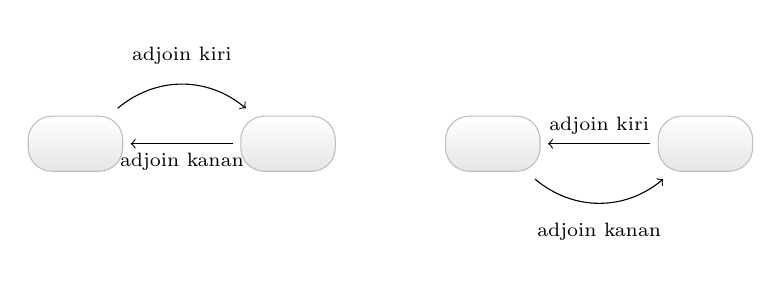
\begin{tikzpicture}[entity/.style={draw, color=black!25, rectangle, rounded corners=3mm, minimum width=12mm, minimum height=7mm, outer sep=1mm, top color=white, bottom color=black!10} ]
		\node[entity] (A) at (0,0) {};
		\node[entity] (B) at (2.7, 0) {};
		\draw (A) edge[->, bend left=40] node[above, inner sep=0.7em]{\scriptsize adjoin kiri} (B);
		\draw (B) edge[->] node[below] {\scriptsize adjoin kanan} (A);

		\node[entity] (C) at (5.3, 0) {};
		\node[entity] (D) at (8, 0) {};
		\draw (C) edge[->, bend right=40] node[below, inner sep=0.7em]{\scriptsize adjoin kanan} (D);
		\draw (D) edge[->] node[above] {\scriptsize adjoin kiri} (C);
	\end{tikzpicture}\end{center}
	Semua isomorfisme adjoin yang terlibat berasal dari Teorema \ref{prop:Hom-tensor-adjunction}.
\end{corollary}
\begin{proof}
	Pembuktian untuk modul kiri dan kanan sama; berikut hanya ditinjau modul kiri ${}_R M$, ${}_S N$. Lemma \ref{prop:forgetful-as-tensor-Hom} bersama Teorema \ref{prop:Hom-tensor-adjunction} menyiratkan
	\begin{align*}
		\Hom\left( {}_R M, {}_{R \to S} \mathcal{F} ({}_S N) \right) & \simeq \Hom\left( {}_R M, \Hom({}_S S, {}_S N) \right) \\
		& \simeq \Hom\left( S \dotimes{R} M, {}_S N \right)
	\end{align*}
	dengan setiap langkah merupakan isomorfisme kanonik. Jadi, diperoleh relasi adjoin $(S \dotimes{R} -, {}_{R \to S} \mathcal{F})$. Demikian pula,
	\begin{align*}
		\Hom\left({}_{R \to S} \mathcal{F} ({}_S N), {}_R M \right) & \simeq \Hom\left( {}_R S \dotimes{S} N, {}_R M \right) \\
		& \simeq \Hom\left( {}_S N, \Hom( {}_R S, {}_R M) \right),
	\end{align*}
	dan setiap langkah merupakan isomorfisme kanonik. Ini membuktikan pernyataan.
\end{proof}

Untuk homomorfisme gelanggang $f: R \to S$ yang diberikan, fungtor-fungtor dalam Korolari \ref{prop:IP-vs-F} juga ditulis sebagai \index[sym1]{P_RS@$P_{R \to S}$}\index[sym1]{I_RS@$I_{R \to S}$} \index{perubahan basis@perubahan basis (base change)}
\begin{gather*}
	P_{R \to S} := - \dotimes{R} S, \quad I_{R \to S} := \Hom(S_R, (-)_R); \\
	{}_{R \to S} P := {}_S S \dotimes{R} -, \quad {}_{R \to S} I := \Hom({}_R S, {}_R (-)).
\end{gather*}
Huruf P mengisyaratkan ``proyeksi'', sedangkan I mengisyaratkan ``induksi''; keduanya jelas merupakan fungtor aditif. Dalam praktik, kita sering memerlukan deskripsi eksplisit dari isomorfisme adjoin di atas. Sebagai contoh, untuk pasangan adjoin $({}_{R \to S} P, {}_{R \to S}\mathcal{F})$, isomorfisme dalam pembuktian, jika dijabarkan dari definisinya, adalah
\begin{equation}\label{eqn:IP-adjunction-explicit-1} \begin{tikzcd}[row sep=small]
	\Hom\left( {}_R M, {}_{R \to S} \mathcal{F} ({}_S N)\right) \arrow[r, "\sim"] & \Hom\left( {}_R M, \Hom({}_S S, {}_S N) \right) \arrow[r, "\sim"] & \Hom\left( S \dotimes{R} M, {}_S N \right) \\
	f \arrow[mapsto, r] & \left[ m \mapsto [s \mapsto s(mf)] \right] \arrow[mapsto, r] & \left[ s \otimes m \mapsto s(mf) \right] ;
\end{tikzcd}\end{equation}
Kasus modul kanan serupa. Ini adalah rumus yang sering digunakan dalam perhitungan dengan hasil kali tensor.

\begin{lemma}\label{prop:IP-transitivity}
	Tinjau homomorfisme gelanggang $\begin{tikzcd} Q \arrow[r, "f"'] \arrow[rr, bend left=25, "gf"] & R \arrow[r, "g"'] & S \end{tikzcd}$. Fungtor pelupa terkait memenuhi persamaan
	\begin{gather*}
		\mathcal{F}_{Q \to R} \circ \mathcal{F}_{R \to S} = \mathcal{F}_{Q \to S}, \\
		{}_{Q \to R} \mathcal{F} \circ {}_{R \to S} \mathcal{F} = {}_{Q \to S} \mathcal{F};
	\end{gather*}
	sedangkan fungtor $P$, $I$ memenuhi isomorfisme
	\[\begin{array}{ll}
		P_{R \to S} \circ P_{Q \to R} \simeq P_{Q \to S}, & I_{R \to S} \circ I_{Q \to R} \simeq  I_{Q \to S}, \\
		{}_{R \to S} P \circ {}_{Q \to R} P \simeq {}_{Q \to S} P, & {}_{R \to S} I \circ {}_{Q \to R} I \simeq {}_{Q \to S} I.
	\end{array}\]
\end{lemma}
\begin{proof}
	Kasus fungtor pelupa $\mathcal{F}$ jelas. Sisanya mengikuti dari Korolari \ref{prop:IP-vs-F} dan sifat komposisi fungtor adjoin (Proposisi \ref{prop:adjunction-composition}); kasus modul kiri dan kanan tentu serupa.
\end{proof}

Sekarang anggap $R$ suatu gelanggang komutatif. Korolari \ref{prop:module-monoidal-cat} menyatakan bahwa $(R\dcate{Mod}, \otimes, \ldots)$ membentuk kategori monoidal. Untuk konsep fungtor monoidal, lihat Definisi \ref{def:monoidal-functor}.
\begin{proposition}
	Bagi homomorfisme $R \to S$ antara gelanggang-gelanggang komutatif, fungtor $P_{R \to S}: R\dcate{Mod} \to S\dcate{Mod}$ mempunyai struktur fungtor monoidal alami.
\end{proposition}
\begin{proof}
	Kita hanya memberikan isomorfisme fungtor $P_{R \to S}(-) \dotimes{S} P_{R \to S}(-) \xrightarrow[\xi]{\sim} P_{R \to S}\left( - \dotimes{R} - \right)$ yang diperlukan bagi fungtor monoidal. Ingat bahwa $P_{R \to S}(M) = M \dotimes{R} S$. Untuk $R$-modul $M$, $N$, definisikan $\xi(M,N)$ sebagai komposisi isomorfisme-isomorfisme berikut:
	\[\begin{tikzcd}[row sep=small, column sep=tiny, every cell/.style={scale=0.93, transform shape, inner xsep=1ex, inner ysep=0.85ex}]
		\left( M \dotimes{R} S \right) \dotimes{S} \left( N \dotimes{R} S \right) \arrow[r, "\sim"] & \left( M \dotimes{R} S \right) \dotimes{S} \left( S \dotimes{R} N \right) \arrow[r, "\sim"] & M \dotimes{R} \left( S \dotimes{R} N \right) \arrow[r, "\sim"] & \left( M \dotimes{R} N \right) \dotimes{R} S \\
		(x \otimes s) \otimes (y \otimes t) \arrow[mapsto, r] & (x \otimes s) \otimes (t \otimes y) \arrow[mapsto, r] & (x \otimes st \otimes y) \arrow[mapsto, r] & (x \otimes y) \otimes st
	\end{tikzcd}\]
	Langkah pertama dan terakhir menggunakan kendala komutativitas $\otimes_R$ (Proposisi \ref{prop:tensor-comm}); langkah-langkah di tengah menggunakan kendala asosiativitas dan kendala satuan $S \dotimes{S} S \rightiso S$ (Proposisi \ref{prop:tensor-unit}). Deskripsi pada baris kedua memudahkan pemeriksaan diagram komutatif dalam Definisi \ref{def:monoidal-functor}, sedangkan syarat $P_{R \to S}(R) = S$ merupakan akibat langsung dari kendala satuan.
\end{proof}
 
